\chapter{Detailed design}
\label{chap:detDesign}


Provide an introduction to the proposed design. This introduction should help
the reader to understand the design choices made.


\section{Interaction Model}
An Interaction Model describes how each \gls{system operation} (that appears in the
Operation Model of the \msrmessir Requirements Analysis Model) is designed to meet
its specification. The design description of each system operation must be
focused on the messages exchanged between the different first-class objects
(i.e. instances of classes either included in Concept Model or introduced as
result of a design choice). An Interaction Model is modeled as a UML Sequence
Diagram.

% 
 \subsection{oeLogin}
 
 \begin{figure}[H]
	\begin{center}
	  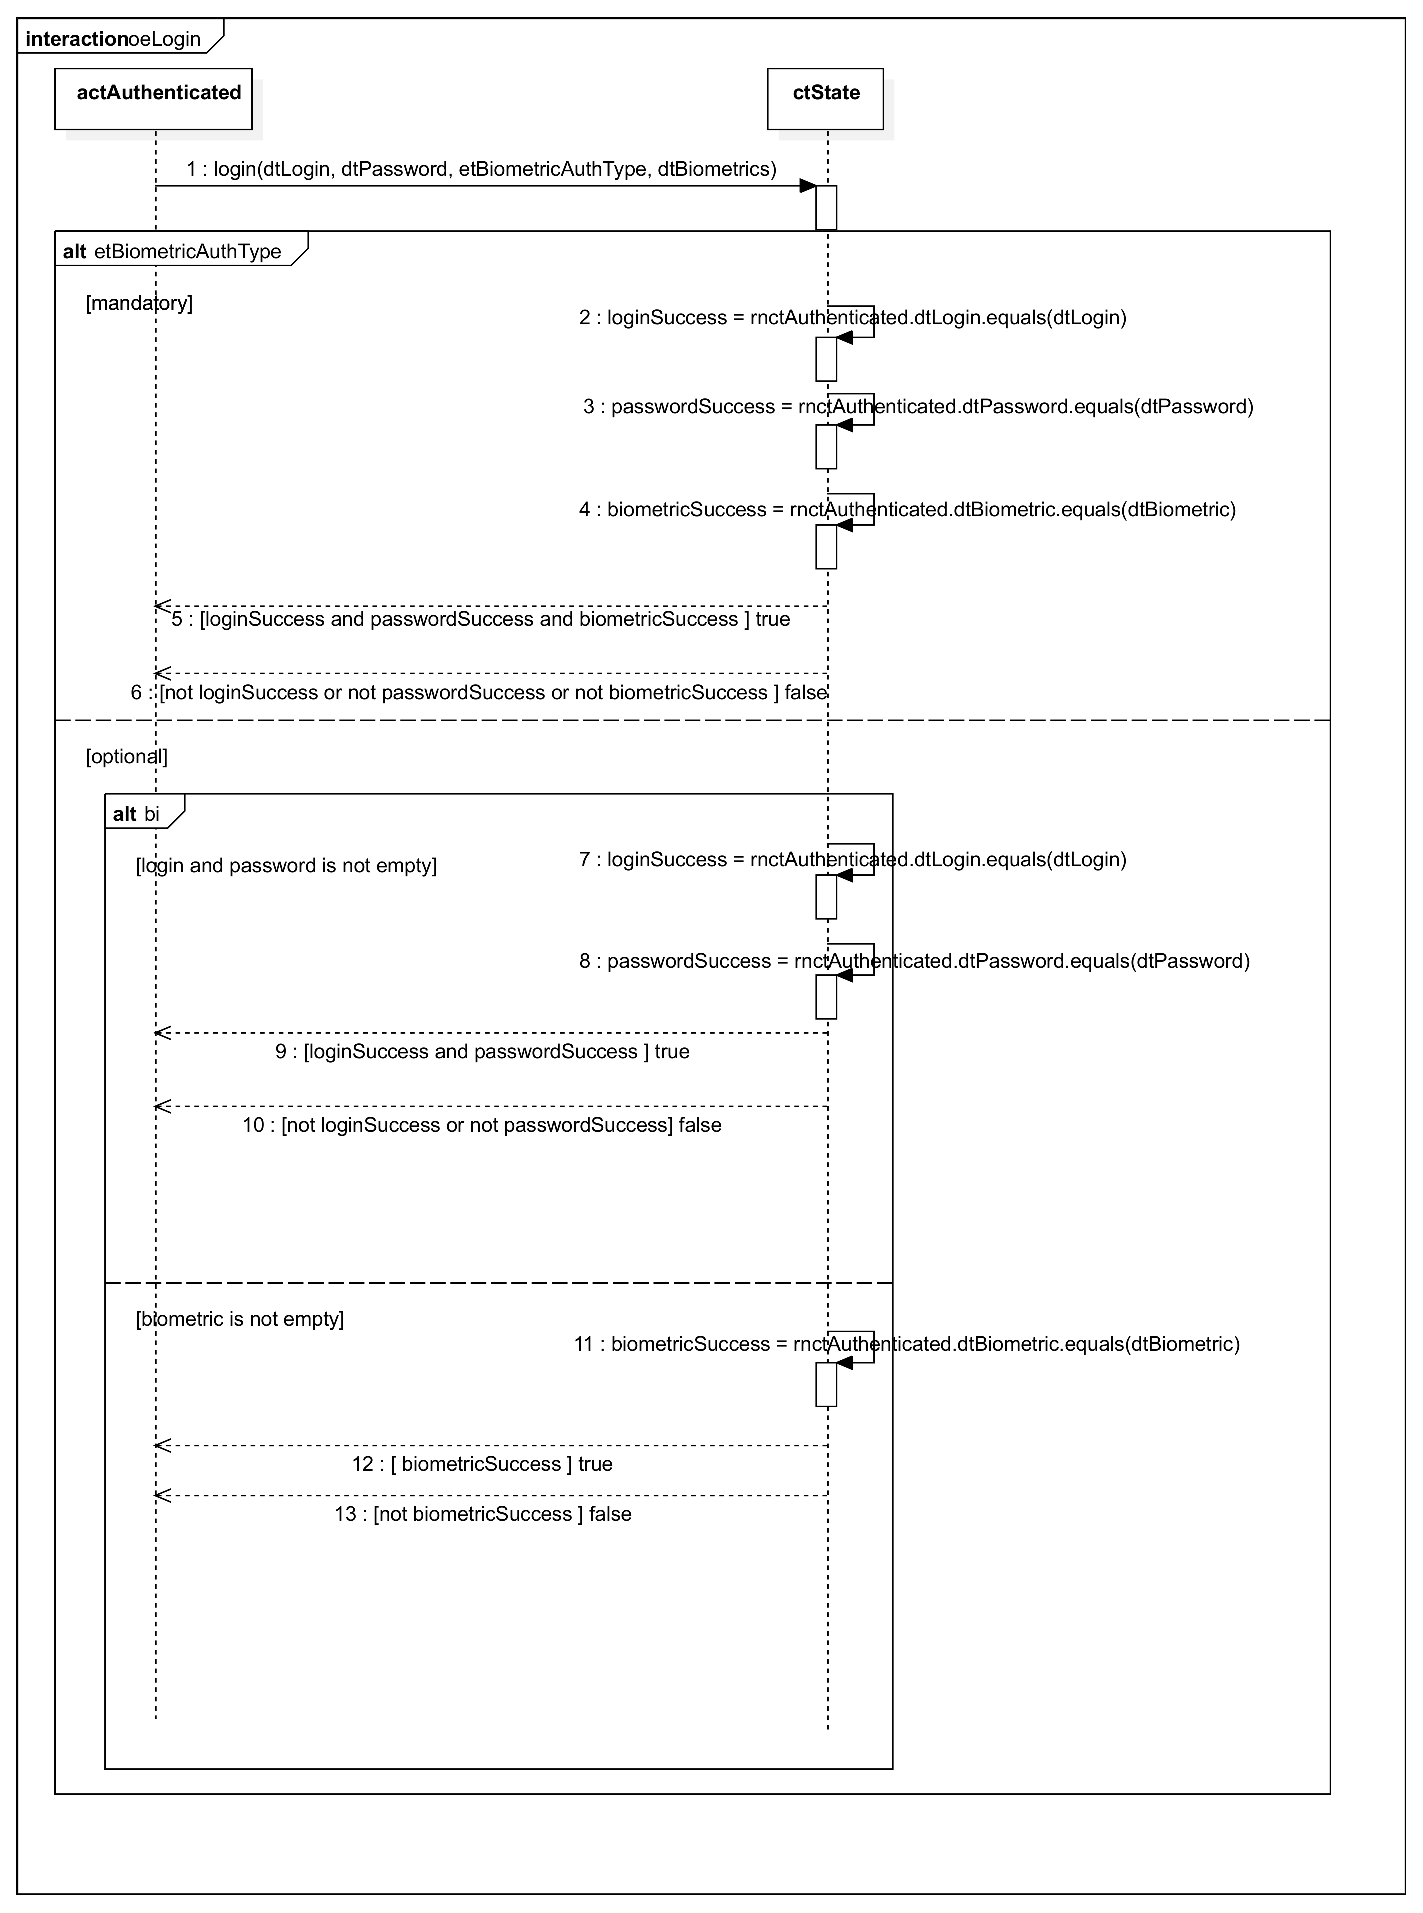
\includegraphics[width=450px]{images/design/login.eps}
	  \caption{Deployment Diagram}
	  \label{fig:deploy-diagram}
	\end{center}
\end{figure}


 \subsection{oeMakeFullReport}
 \begin{figure}[H]
	\begin{center}
	  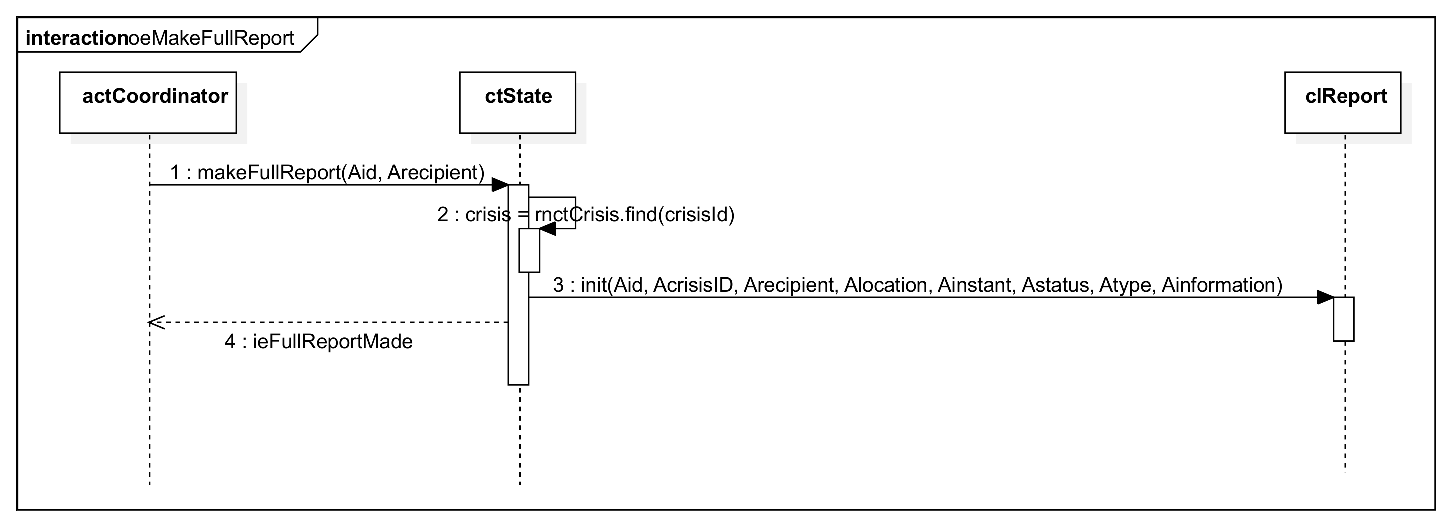
\includegraphics[width=450px]{images/design/makeFull.eps}
	  \caption{Deployment Diagram}
	  \label{fig:deploy-diagram}
	\end{center}
\end{figure}
 
% TODO
% 
% 
% \subsection{oeSystemOperation3}
% TODO



\section{Design Class Model}
The Design Class Model is composed of the contents of all design classes (i.e.
every class appearing in at least one Interaction Model), all the navigable associations between design
classes, and the inheritance structure. The description of each class must
contain its attributes and operations. The Design Class Model is modeled as a
UML Class Diagram. 

It is advised to split the Design Class Model into multiple views as such model
may become pretty large. 
	

%\subsection{Design Class Model view1}
% TODO
% 
% 
% \subsection{Design Class Model view2}
% TODO
% 
% 
% 
% \subsection{Design Class Model view3}
% TODO